%!TEX TS-program = xelatex
\documentclass[]{friggeri-encvblackwhite}
%\addbibresource{bibliography.bib}
%\usepackage{natbib}

\begin{document}
\header{}{Curriculum Vitae}
       {}
% In the aside, each new line forces a line break
\begin{aside}
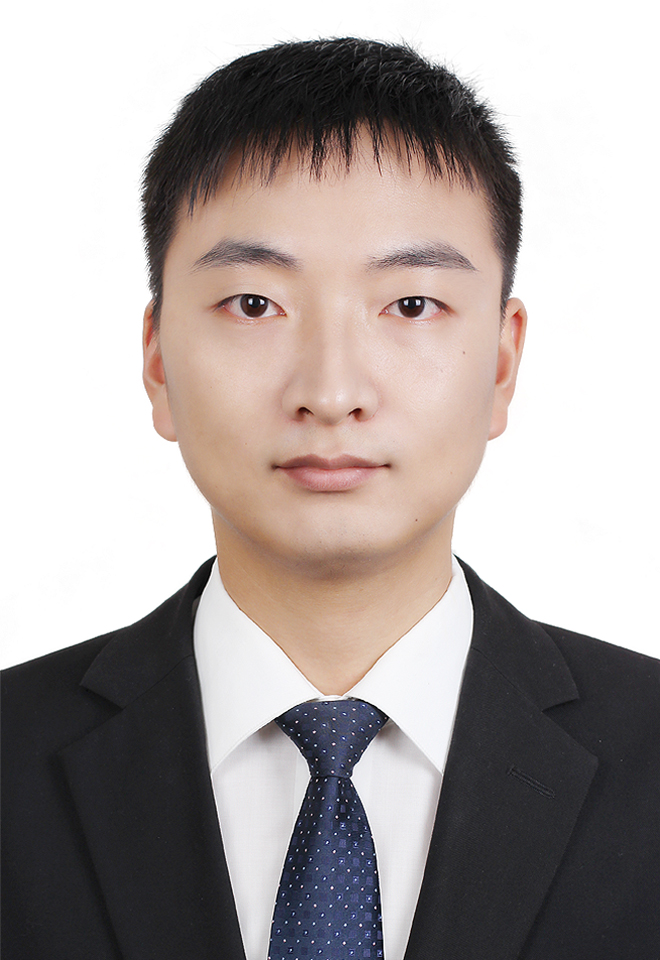
\includegraphics[width=4cm]{IMG_4827small.jpg}
  \section{About}
  Name: Tengfei Wang
  Gender: Male
  Degree: PhD of Geophysics
  E-mail:\quad wang.tengfei0221@gmail.com
%  mail:1110701@tongji.edu.cn
  Address: NO.1239, Yangpu District, Shanghai
  Phone: 18817367538
  \section{Language}
  CET-6:522
  \section{Programming}
	Unix/Linux
    C/C++
	MPI/OpenMP
    Shell/Python/Java
\end{aside}

\section{Special skills}
\large
1. High-performance computing with C through MPI \& OpenMP. \\
2. C++/Python/Java \& Unix/Linux OS \\
3. Large data processing \& Small-cluster maintenance experience. \\
4. Good mathematical background.

\section{Education}
\begin{entrylist}
  \entryTwo
    {2011-2017}
    {PhD. \quad Tongji University \quad Profession: Geophysics}
  \entryTwo
    {2007-2011}
    {B.S. \quad Tongji University \quad Profession: Geophysics}
\end{entrylist}
\section{Research}

\begin{entrylist}
  \entry
    {2010-2011}
	{Local angle domain imaging in azimuthally anisotropic media }
	{\emph{Introduce the Kirchhoff PSTM algorithm for azimuthally anisotropic media in
	local angle domain.}}
  \entry
    {2011-2013}
    {Velocity building with Tomography based on angle gather in depth domain}
    {\emph{Using Gaussian beam migration as engine, combining open-source software to solve large spare matrix 
		in geophysical problem \& parallelizing with OpenMP and MPI\\
	}}
  \entry
    {2013-2015}
    {Elastic FWI based on wave mode decomposition}
    {\emph{
		Precondition the gradient of elastic FWI using decomposed wavefields to 
		mitigate elastic parameter trade-offs through wave mode decomposition.
		Complete algorithm design and programming with hybrid MPI+OpenMP method
		to solve the memory consumption problem. 
	}}
  \entry
    {2015--}
    {Elastic Reflection FWI based on wave mode decomposition}
	{\emph{
		Update the background P- and S- velocities using reflected waves. 
		Mode decomposition is used to mitigate parameter trade-offs both in
		imaging and rabbit-ear gradient calculation.
	}}
\end{entrylist}

\section{Internship}
\begin{entrylist}
  \entry
    {2012-2014}
	{CNPC CDEC Sichuan Geophysical Company}
	{\emph{
		Participate the project of my supervisor and 
		transplant the Tomography algorithm into the platform of their company.
	}}
  \entry
    {2011-2012}
    {Sinopec research center in Nanjing}
	{\emph{
		Participate the project of my supervisor and take responsibility to the
		test and transplantation of the algorithm. Complete part of the algorithm
		optimization.
	}}
\end{entrylist}
\section{Honor}
\begin{entrylist}
  \entryTwo
    {2011}
    {Geophysical scholarship of Liu Guangding}
  \entryTwo
    {2012}
	{The Graduate National scholarship}
  \entryTwo
    {2013}
    {Geophysical scholarship of Tongji University}
\par\vspace{\parskip}
%\vspace{3cm}
\end{entrylist}

\section{International experience}
\begin{entrylist}
  \entry
    {2016}
    {3-month visit in King Abdullah University of Science and Technology}
	{\emph{
	}}
  \entry
    {2016}
    {EAGE annual meeting}
	{\emph{Oral Presentation: Comparison between mode decomposition based and Gaussian Newton methods in
		elastic full waveform inversion
	}}
  \entry
    {2015}
    {EAGE annual meeting}
	{\emph{Oral Presentation: 
		Elastic wave mode decoupling for full waveform inversion
	}}
  \entry
    {2012}
    {SEG annual meeting}
	{\emph{Oral presentation: Pure mode modeling and reverse-time migration of P-wave in
		HTI and orthorhombic media
	}}
\end{entrylist}
\section{Jounal Articles}
\begin{entrylist}
  \entry
    {2017}
	{Geophysical Journal International: Elastic full waveform inversion based on mode
		decomposition: The approach and	mechanism 
	}
	{\emph{Tengfei Wang, Jiubing Cheng}}
  \entry
    {2014}
	{Chinese J. Geophysics: Description of qP-wave propagation in anisotropic media, 
		Part II: Separation of pure-mode scalar waves.}
	{\emph{Jiubing Cheng, Chen Maogen, Tengfei Wang}}
  \entry
    {2013}
	{Chinese J. Geophysics: Description of qP-wave propagation in anisotropic media, 
		Part I: Pseudo-pure-mode wave equations.}
	{\emph{Jiubing Cheng, Kang Wei, Tengfei Wang}}
  \entry
    {2012}
    {Geophysics: Azimuth-preserved local angle-domain prestack \\
    time migration in isotropic vertical transversely isotropic\\
    and azimuthally anisotropic media}
    {\emph{Jiubing Cheng, Tengfei Wang, Chenglong Wang, Jianhua Geng}}
\end{entrylist}
\section{Conference Abstracts}
\begin{entrylist}
  \entry
    {2017}
	{87th SEG Annual meeting: Born reflection kernel analysis and wave-equation reflection
	traveltime inversion in elastic media}
	{\emph{Tengfei Wang and Jiubing Cheng }}
  \entry
    {2017}
	{79th EAGE Annual meeting: Elastic wave-equation reflection traveltime inversion
	using dynamic warping and wave mode decomposition}
	{\emph{Tengfei Wang, Jiubing Cheng, Chenlong Wang and Qiang Guo }}
  \entry
    {2016}
	{78th EAGE Annual meeting: Comparison between mode decomposition based and Gaussian
	Newton methods in elastic full waveform inversion}
	{\emph{Tengfei Wang and Jiubing Cheng}}
  \entry
    {2016}
	{SPG/SEG 2016 International Geophyisical Conference: Regularization method of 
	tomography based on the ADCIGs 	with geological dip information}
	{\emph{Tao Yang, Tengfei Wang and Jiubing Cheng }}
  \entry
    {2015}
	{77th EAGE Annual meeting: Elastic wave mode decoupling for full waveform
	inversion}
	{\emph{Tengfei Wang and Jiubing Cheng }}
  \entry
    {2014}
	{SPG/SEG 2014 International Geophyisical Conference: Migration velocity model building 
	using local angle domain nonlinear tomography.}
	{\emph{Tengfei Wang, Kang Wei and Jiubing Cheng }}
\end{entrylist}

\end{document}
